\chapter{Project Management & DevOps}\label{DevOps}

\section{Project Organization}

As part of a Multi-Agent System ourselves, we needed to establish some formal organization and communication channels that were of utmost importance for the progress of the project.

\subsection{Communication}

Our main source of organization was through in-person and online meetings, both General and Team-Based ones.

Apart from having weekly meetings, we decided to use \texttt{Slack} as the main channel for global and intra-team communications.
Each sub-team had a separate channel to communicate, discuss and share ideas that could be brought up for discussion on the general meetings we had so that a final decision was made.

As far as dispute resolution is concerned, in most cases we went with majority voting upon the ideas that were up for discussion. In some other occasions (such as General Rules and Conventions) we went with general consensus: ideas where brought up and if no one objected, those were added to the list of rules/conventions we needed to follow.

\subsection{Documentation}

Each sub-team was responsible for keeping up-to-date documentation of what has been implemented/agreed upon as a reference for everyone on the project (e.g., Overview Documentation, Maths Documentation, Infrastructure MVP and Quick Start Documentation)

\subsection{Rules \& Conventions}

In order for us to effectively work in parallel towards accomplishing our common goal (i.e., develop a platform where agent strategies could be formed as to escape the pit) we had to agree and decide upon some General Rules and Conventions.
Those included General Project Management Rules, Coding and Reporting Conventions both of which are publicly available on the main page of our projects' repository.

\subsection{Programming Language}

Upon voting the majority agreed to use the programming language of Go. That decision was heavily influenced by Go's ability to implement concurrency which was a desired feature for the Peer-2-Peer communication level between the agents. Some other important factors were previous years' implementations and package managing implemented within Go (with go.mod).

\newpage

\section{Project Management}

One of the most crucial parts in any Software Engineering Project is effectively tracking changes on files. As a solution to that we have utilised Git as a Version Control System and GitHub as the online counterpart.

\subsection{GitHub}

The code repository can be found on: \url{https://github.com/SOMAS2022/SOMAS2022}

We have created 2 repositories: One for hosting the code of our Environment and Agents' implementations and one for the Final Report of the Project.

On those repositories, each team (either sub-teams or agent teams) should create a separate branch for a specific feature and work on it. After the implementation was done they would have to create a Pull Request to merge the changes to the main branch. We have agreed to use branch protection on the main branch and each merge was only possible after it has been reviewed by at least another member that was not involved in the implementation of that specific feature, to ensure code integrity and readability.

\subsection{Project Progress}

In order to track Project Progress and Task Allocation we have used GitHubs' Issues feature. 
Through that functionality we were able to Create and List Tasks that needed to be done by hierarchically ordering them according to importance and team-specific labels.
Moreover, through the assignment of Milestones we were able to monitor deadlines and keep delegation of work on time.
Last but not least, members of the Infrastructure Team could self-assign to a single (or multiple) issue which helped improve the efficiency and transparency for each task.

\newpage

\section{DevOps}

The foundational idea behind the DevOps Team was to make the implementation process easily accessible to everyone while ensuring that the "quality" and integrity of code, according to communally agreed upon "best practices", created at any step was not violated. These considerations stemmed from the fact that many people in teams had little programming experience and/or little to no Golang experience. This was accomplished through various Continuous Integration - Continuous Deployment (CI-CD) methods:

\subsection{GitHub Actions}

GitHub Actions are a GitHub feature that allows for the automation of repetitive tasks, such as building, testing, and deploying code, thus making it a powerful tool for automating development workflows. We used this as not only does it save time and effort for teams, but it also helps to ensure that the software is always in a deployable state. With automated builds and tests, the agent teams can focus on developing and testing their agents, rather than worrying about manually running builds and tests every time they make a change, or having to use Linux scripting tools they might not be used to.

GitHub Actions allows for the creation of custom workflows that are triggered by specific events, in our case  the creation of a new branch or the opening of a pull request. This allowed us to automate the review process, ensuring that code is tested before everyone reviews it and it gets merged to the main branch.

As part of our workflow, our code was complied and our tests were automatically run, but also any changes went through linting, deadlock detection, and cyclic reference checking:
\begin{itemize}
    \item Linting helped us find syntax errors, formatting issues, and potential bugs, which make code easy to read, while increasing its quality and maintainability.
    \item Deadlock detection allowed us to identify and prevent situations where two or more channels are waiting for resources that are held by the other channels, which is critical to our system due to our heavy use of concurrency. This increased the performance by avoiding indefinite loops and the reliability by avoiding our program timing out. 
    \item Cyclic reference checking let us detect and resolve circular references in data structures, which directly improved memory usage, reliability and maintainability. 
\end{itemize}


From a self-organizing perspective, another benefit of using GitHub Actions is that it provides a centralized, non-biased and consistent way to manage the software development process across the infrastructure team. With comments about errors and mistakes now automated, interpersonal conflicts arising due to arguments are now automated away!

% Linting 
% Deadlock
% Cyclic refference
% Report Copmilation on report repo


\subsection{(Unit) Testing}

Due to the heterogeneous nature of our project, due to the different implementations of each agent team, our testing strategy consisted of unit testing, i.e. testing individual units of code at the function or module level for proper behavior. This was to ensure that despite any code change, our core infrastructure functionality would function. This allowed teams to delve deeper into their agent testing and self-organizing ideas as our core code base was now more maintainable and robust.

For example, all our core math equations (eg: calculating the monsters damage dealt) have their own associated unit tests that cover edge cases. This ensures the repeatability and reliability of our infrastructure. 

%Moreover, all our basic agent functionalites
% Math equation check
% Basic Agent Functionalities

\subsection{Scripts/Deployment}

We used makefiles (from GNU Make) to automate the build process for software project. This abstracted away the Linux experience required to build such a project by allowing people to compile the entire project in one word (make!). From a DevOps perspective, this ensured reliability of the compilation process  and improved the efficiency as compilation, testing, running, cleaning the environment and more were all abstracted away.  

However, due to some users using a windows OS based platform and thus not having access to Linux commands, we usually recommended them to use Windows Subsystem for Linux (WSL), and provided additionally a docker container. 

Docker containers allowed us to extend the benefits of using makefiles to all platforms. After sharing and building our docker container, everyone now had access to a shared standardized environments for building and testing on our project. 

Also in our mind during the early DevOps development phases, this Docker container was also created to enable us to potentially scale our project very large and very fast for massive experiment purposes.

% Docker container
% Makefile

\subsection{Package management}

Our  programming language Go was also picked for its DevOps advantages, more specifically when it comes to package management, which is very prone to many issues such as bugs and unreliability. This combined with Go's fast compile times creates a fantastic development environment for everyone to use. 

Firstly, Go has a built-in dependency management system that allows us to specify the dependencies of their packages in a standardized way, which makes it easy to manage and update dependencies as needed, and most importantly, consistent across all members. 

Go's dependency management system also includes support for versioning, which allows us to specify the specific version of a dependency that a package requires, again ensuring reliability of the project.

Finally, Go has a centralized package repository, which ensures that all packages used come from a single, authoritative source,  once again ensuring consistency, reliability and increasing security in our project.

\newpage

\section{Project Structure}

Following common coding practises in Go and project structures from previous years as our main inspiration, we came up with the following structure \ref{fig:proj_struct}:

\begin{figure}[h]
    \centering
    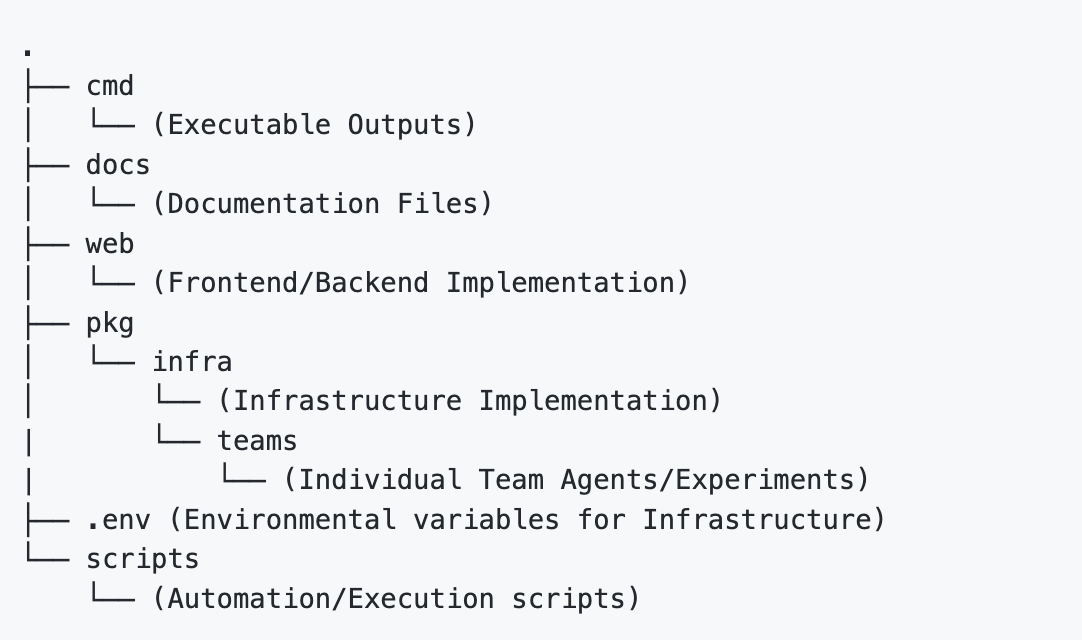
\includegraphics[width=0.8\textwidth]{figures/proj_struct.png}
    \caption{Project Structure}
    \label{fig:proj_struct}
\end{figure}